\section{Domain Analysis}\label{sec:domainAnalysis}
In this section, we specify our blazar observation data and define domain-specific goals and visualization tasks that were identified in consultation with our domain experts. 

\subsection{Blazar Observation Data}\label{sec:BlazarData}
Multiple observatories worldwide collect blazar data; however, their observed properties or units of measurement differ depending on the telescopes being used. 
%are different depending on the used telescopes.
To reduce uncertainties due to missing observational data and observation errors,
TimeTubesX allows users to fuse multiple datasets for the same blazar from different observatories 
through the automatic handling of potentially different definitions of observed variables~\cite{Fujishiro2018}.
Thus, users can, for example, include data from Hiroshima University and the University of Arizona in the same visualization session. 
TimeTubesX is designed to primarily process datasets acquired by the Hiroshima Astrophysical Science Center at Hiroshima University,
which uses a $1.5\mathrm{m}$ Kanata telescope. 
%taking full care of discrepancy in the definition of variables~\cite{Fujishiro2018}.

% Observation datasets
The photometric and polarimetric datasets of Hiroshima University include six time-dependent variables: $q$, $u$, $\epsilon_q$, and $\epsilon_u$ for polarization (Fig.~\ref{fig:blazar} (A)), $I$ for intensity (Fig.~\ref{fig:blazar} (B)), and $C$ for color (Fig.~\ref{fig:blazar} (C)).
%which are illustrated in the lower part of \autoref{fig:blazar}.
% Astronomers use Julian Day for timestamps of observations. 
% Our domain experts mainly use $t = \rm{Julian\,Day} - 2{,}450{,}000$ instead of the original Julian Day for simplicity.
Linear polarization is represented by $Q$ and $U$, the so-called \textit{Stokes} parameters.
$I$ denotes the observed intensity of the light.
% i.e., the total of the luminosity of polarized components ($polarized\,flux$) and that of unpolarized components ($unpolarized\,flux$).
We mainly use fractional values of $Q$ and $U$ where $q = Q / I$ and $u = U / I$, 
because $q$ and $u$ describe the behaviors of a blazar more effectively than $Q$ and $U$~\cite{Uemura2016}.
We call the plane composed of $q$ and $u$ the \textit{Stokes plane}.
$\epsilon_q$ and $\epsilon_u$ act as the observation errors of $q$ and $u$, respectively.
$C$ denotes the observed color of a blazar.
The polarization degree ($PD$) and polarization angle ($PA$) derived from $q$ and $u$ are used to describe the optical polarization.
$PD$ denotes a distance from the origin of the Stokes plane, 
while $PA$ denotes one half of the polar angle in the Stoke plane, as illustrated in Fig.~\ref{fig:blazar}~(A).

% HOW MANY SAMPLES PER DAY
% THE TYPICAL SIZE OF ONE DATA
% HOW MANY DATASETS
The observation frequency differs depending on observatories.
The median observation interval of Hiroshima University is once every two days.
% while that of the University of Arizona is once a day.
Note that the datasets have missing data due to the rotation and/or revolution of the Earth, bad atmospheric conditions, and so on.
% Our primary datasets from Hiroshima University include about 300 to 400 data samples from the years 2008 to 2014. 
In this paper, we process datasets from Hiroshima University for two blazars: \emph{BL Lac} and \emph{3C 454.3}. 
The two datasets for \emph{BL Lac} contain 285 data samples in each dataset from May 2008 to December 2011, while the one for \emph{3C 454.3} contains 355 data samples from July 2008 to July 2014.
% \begin{eqnarray}
% PD(t) & = & \sqrt{q(t)^2+u(t)^2}, \label{equ:PD}
% \label{eqn:PD}\\
% PA(t) & = & \frac{1}{2} \rm{arctan}\left(\frac{u(t)}{q(t)}\right). \label{equ:PA}
% \end{eqnarray}

% TimeTubesX is a joint research project carried out by computer scientists in the visualization group at Keio University 
% and astronomers in Hiroshima Astrophysical Science Center at Hiroshima University,
% so we currently work with datasets from Hiroshima University,
% $q$ and $u$ imply the polarized flux portion of the total flux.
% The relations among the polarization parameters are illustrated in the lower left part of \autoref{fig:blazar}. 
% $C$ denotes the observed color of a blazar.
% The smaller $C$ value is, the bluer the light from a blazar is. 
% Conversely, the larger $C$ value is, the redder the light is.
% The astronomers need to correlate the polarization, intensity, and color of the light from blazars
% to understand the behaviors of blazars.

\begin{figure}[tb]
    \centering
        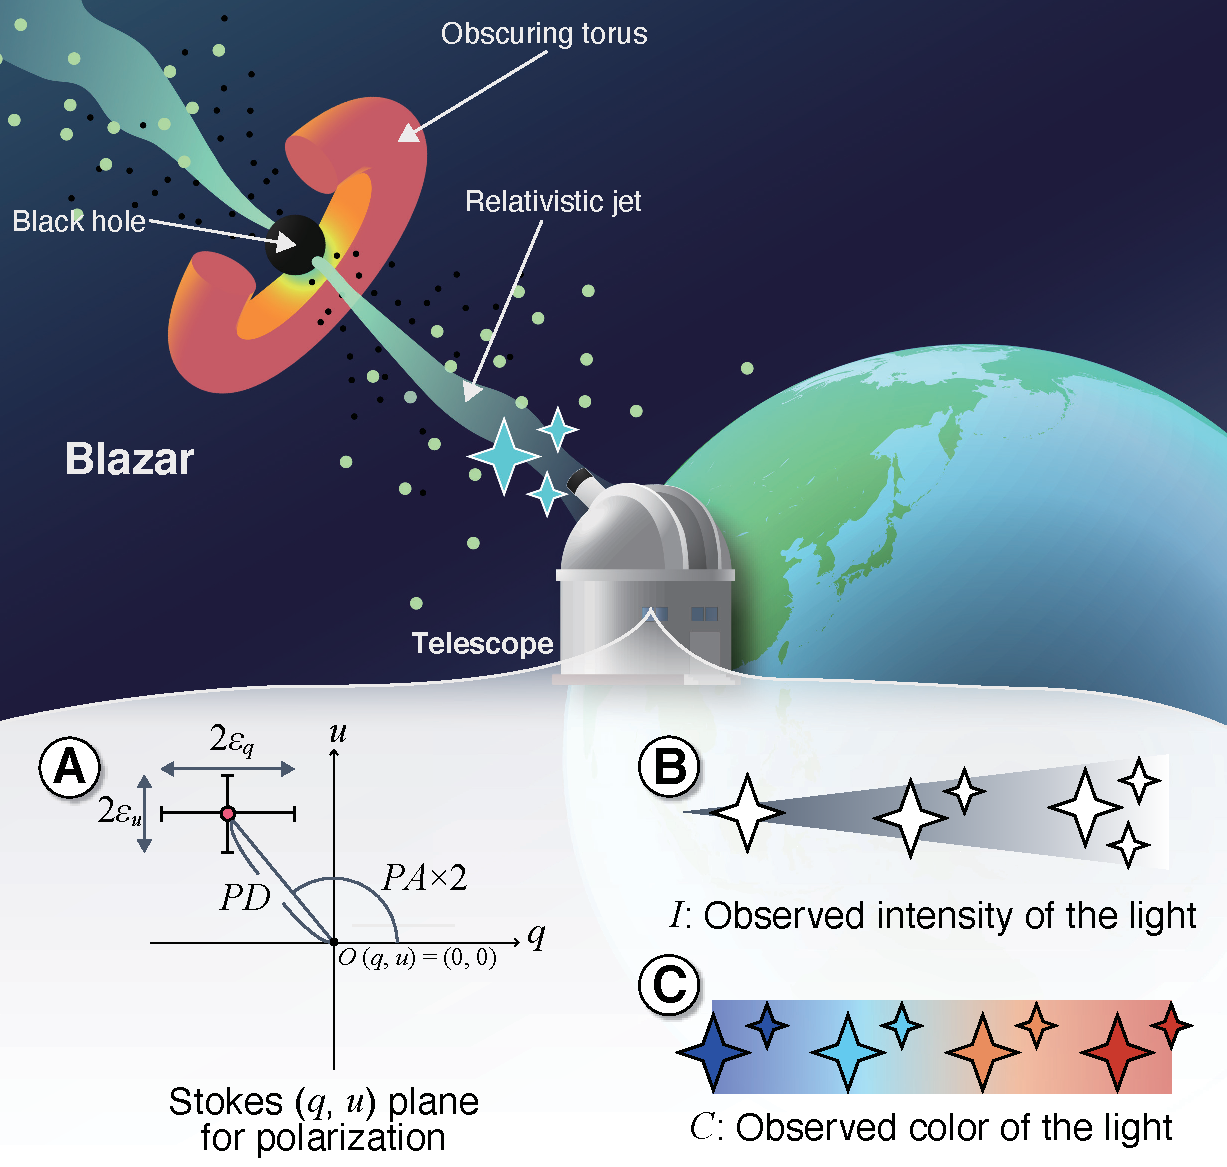
\includegraphics[width=.99\linewidth]{vgtc_journal_latex/figures/blazar_final.pdf}
    \caption{An observed blazar and its features. A blazar's central black hole emits a relativistic jet toward the Earth.
        The telescope observes its light in terms of (A) polarization, (B) intensity, and (C) color.}
    \label{fig:blazar}
\end{figure}

\subsection{Goals and Visualization Tasks}\label{sec:domainGoalsandTasks}
% \begin{figure}[tb]
%     \centering
%     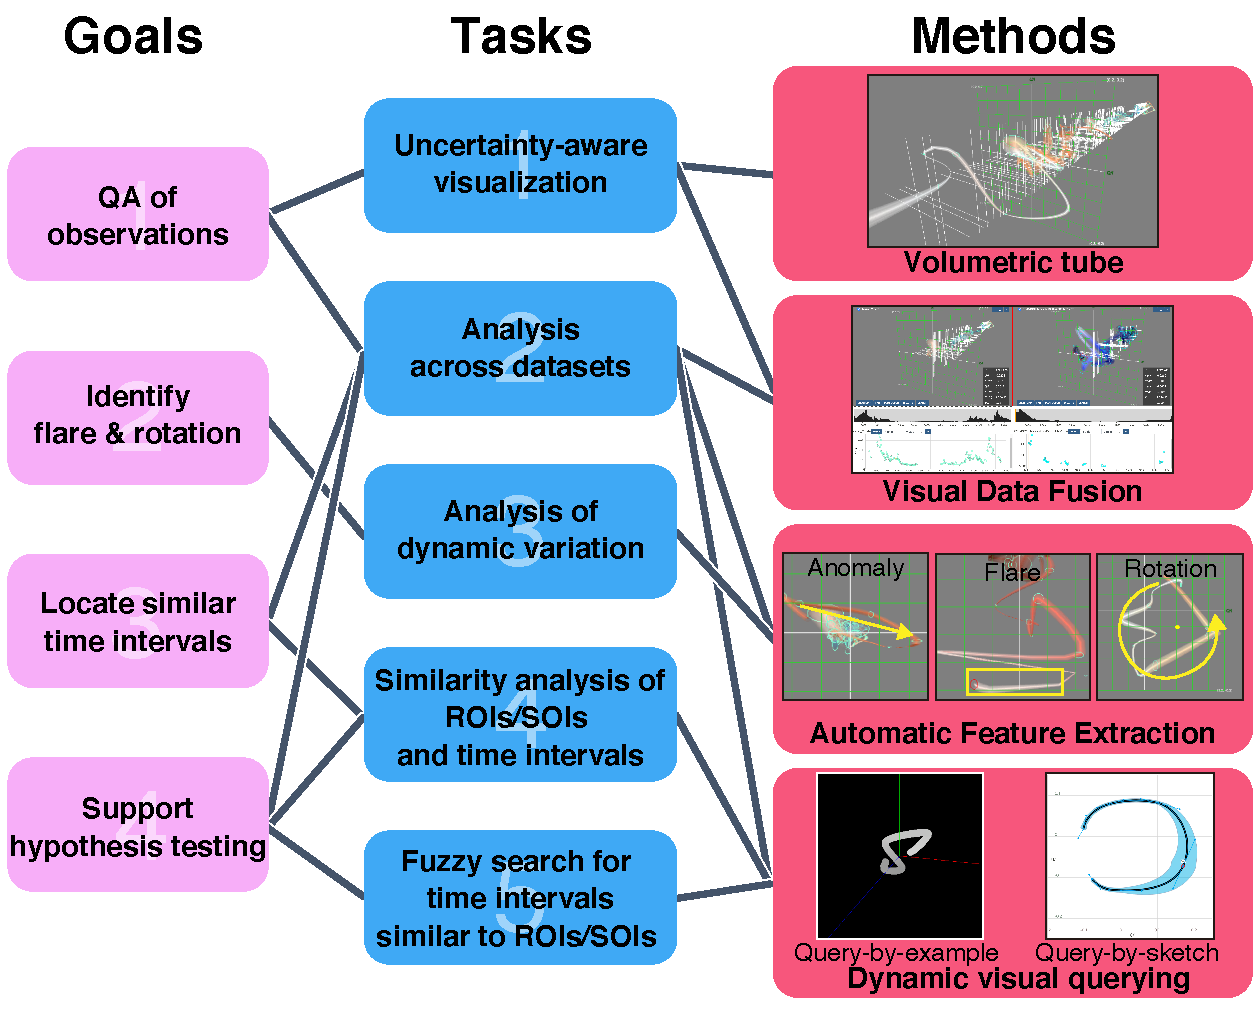
\includegraphics[width=.99\linewidth]{vgtc_journal_latex/figures/many-to-many.pdf}
%     \caption{Mapping of four domain goals, five time-series data analysis tasks, and four functions of TimeTubesX.}
%     \label{fig:mapping}
% \end{figure}
We interviewed two astronomers at Hiroshima University, one at Stanford University, and four at Boston University to clarify the domain goals and visualization tasks.
% which has nine blazar researchers.
The main objective of these astronomers is 
to quickly extract and analyze features in temporal variations of observed polarization, intensity, and color that are occurring at multiple time intervals. 
TimeTubesX effectively supports the following four domain goals:

\noindent\textbf{G1--Enhance the reliability of blazar observations}. 
% Due to the rotation of the Earth or bad atmospheric conditions, 
Datasets always contain missing data and observation errors. 
Astronomers need to assess whether what they have found is plausible by analyzing the length of missing data periods and the size of errors.

\noindent\textbf{G2--Identify flares and rotations}. 
Astronomers typically pay attention to time intervals with dynamic time variations, %features that dynamically change over a period of time. 
% Examples include 
such as flares and rotations.
% such as flares that occur when the blazar is more energetic than usual and polarization rotations. %, which sometimes co-occur with dynamic changes of $I$ or $C$.
The analysis of time intervals with such dynamic variations helps astronomers demystify jets' structures.
% For example, astronomers are interested in polarization variations at the time of flares.
% These dynamic behaviors are important because they help astronomers demystify the jet's structures.

\noindent\textbf{G3--Locate recurring blazar behaviors}.
Besides well-known behaviors such as flares and rotations, 
recurring patterns or common features can also exist.
Thus, upon finding an interesting pattern or feature, 
astronomers want to locate other time intervals similar to it.

\noindent\textbf{G4--Explore time intervals validating a hypothesis of blazar behaviors}.
Through their analyses or experiences, astronomers sometimes make a hypothesis (e.g., that the flares of a blazar tend to co-occur with a specific polarization variation pattern). 
Astronomers need to address time intervals that might validate the hypothesis.

% \begin{enumerate}[nosep, label=\textbf{G\arabic*}, align=parleft, leftmargin=*]
%     \item Enhance the reliability of observations;
%     \item Identify flares and rotations;
%     \item Locate time intervals similar to a specific region/shape of interest (\textit{ROI} or \textit{SOI});
%     \item Explore time intervals validating specific hypotheses.
% \end{enumerate}

To attain these goals, we have identified five visualization tasks that TimeTubesX should support:

\noindent\textbf{T1--Uncertainty-aware visualization.} 
% Due to bad atmospheric conditions or the rotation of the Earth, datasets will always contain observation errors and missing data. 
% Astronomers need to assess whether the interesting behavior they found is plausible or not by analyzing the size of observation errors and the length of missing data periods.
Users should be able to perceive the reliability of data through visualizations. 

\noindent\textbf{T2--Analysis across datasets.} 
% Combining datasets from multiple observatories can reduce the effect of observation errors and compensate for missing data. 
% Additionally, some astronomers want to extract features over several datasets.
%On the other hand, some astronomers think there can exist a universal feature among multiple blazars.
To compensate for missing data, 
the system must allow users to aggregate datasets for the same target from different sources.
Analyses across datasets should also be supported to address features that are common to multiple targets.

\noindent\textbf{T3--Analysis of dynamic variations.} 
% Astronomers typically want to identify time intervals with dynamic changes. %features that dynamically change over a period of time. 
% Examples include flares, when the blazar is more energetic than usual, or polarization rotations, which sometimes co-occur with dynamic changes of $I$ or $C$.
Time intervals with drastic changes in a short time period and those with unusually large time variations should be automatically extracted.
% Users want to investigate drastic temporal changes over a few days and large changes in values.
% or a sudden change in the polarization angle.
%The rotation of polarization is also interesting to them. 
% Some astronomers think rotations tend to co-occur with dynamic changes of $I$ or $C$. 
% Thus, TimeTubesX supports the analysis of dynamic variations of polarization, intensity, and color by incorporating different feature extraction on querying methods. %can be observable blazar behaviors.

\noindent\textbf{T4--Similarity analysis of a specific region/shape of interest and time intervals.} 
% When finding an interesting pattern, 
% % When finding an interesting behavior/pattern or confirming a hypothesis, 
% astronomers want to find other time intervals similar to the pattern. 
% This requires the ability not only to identify ROIs/SOIs, but also to search for similar data points.
% , either by the automatic feature detection or dynamic visual queries.
Users should be able to identify regions/shapes of interest (\emph{ROI}s/\emph{SOI}s) and search for similar time variation patterns at other time intervals without using complex query languages or parameter settings.
% The system should allow users to build a query for a ROI/SOI without complex query languages or parameter settings.

\noindent\textbf{T5--Fuzzy search for time intervals similar to a specific ROI/SOI.}
%A prerequisite for similarity analysis between similar time intervals is the ability to detect similar intervals.
%Astronomers are not only interested in finding highly similar time intervals, 
% Astronomers are interested not only in exact matches between a ROI/SOI and similar time intervals, but also in fuzzy or approximate matches. 
% For example, they need to find time intervals that have similar time variations to the ROI/SOI, but are in a different scale or at a different position on the Stokes plane.
% A single query can be produced under different mental models.
The system should provide not only exact matches between a ROI/SOI and time intervals but also fuzzy or approximate matches. 
%There exist time intervals which have similar time variations but in a different scale or at different position on the Stokes plane. 
%The astronomers want to distinguish among these.

% Our previous work~\cite{Fujishiro2018}, TimeTubes, has already supported the first two tasks.
% To support \textbf{G1},
% we have proposed the 3D volumetric tube visualization,
% which allows users to perceive uncertainties of observations (\textbf{T1}).
% % The volumetric tube visualization itself makes users perceive uncertainties of observations (\textbf{T1}). 
% The vagueness of the tube's appearance allows users to recognize the reliability of data samples.
% An ellipsoidal snapshot and a white cruciform axis appear at each observation time stamp to distinguish missing data.
% To ameliorate the ambiguities caused by missing data or observation errors (\textbf{G1}), we have introduced the visual data fusion, which allows users not only to aggregate multiple datasets for the same blazar but also to effectively compare multiple datasets for the same/different blazar in a single visualization session (\textbf{T2}).
% To achieve the remaining goals (\textbf{G2}, \textbf{G3}, \textbf{G4}),
% TimeTubesX also supports \textbf{T3}, \textbf{T4}, and \textbf{T5} by incorporating automatic feature extraction and dynamic visual querying.
% , as we will explain in the rest of the paper.
To support \textbf{G1}, our previous work, TimeTubes~\cite{Fujishiro2018}, has already supported \textbf{T1} and \textbf{T2}.
Observation errors are encoded in the appearance of the 3D volumetric tube (\textbf{T1}).
An ellipsoidal snapshot and a white cruciform axis appear at each observation time stamp to distinguish missing data (\textbf{T1}).
Analysis across datasets (\textbf{T2}) is supported by visual data fusion, which allows users not only to aggregate multiple datasets for the same blazar but also to effectively compare multiple datasets for the same or a different blazar in a single visualization session.
In this paper, we mainly focus on feature and pattern detection methods to support the remaining tasks (\textbf{T3}, \textbf{T4}, \textbf{T5}).
Consequently, we have designed an integrated visual analytics framework for blazar observations that supports all identified goals (\textbf{G1}-\textbf{G4}) and tasks (\textbf{T1}-\textbf{T5}).


% So, they want to query ROI or test their hypothesis across datasets for multiple different blazars.
% If they can find such time variations, the behavior or hypothesis can be reported as a new feature.
% ROI querying

% \textbf{T3 -- Hypothesis test.} Universality between behaviors is the most important factor for astronomers. 
% Through their analyses or experiences, they sometimes build a hypothesis. 
% To verify the hypothesis, they scrutinize time intervals satisfying it.
% Their shapes look similar but inherently different. 
% Time variations of data samples on the Stokes plane are affected by other polarization components in the universe. 
% There can exist time intervals with a similar shape to other time interval but in the different position of the Stoke plane.
% The position of the rotation center is not consistent. 
% For example, one rotation starting from the origin of the Stoke plane may move to the upper right and then come back to the origin in a counterclockwise direction, 
% while other rotation starting from the origin of the Stoke plane may move to the lower left and then come back to the origin in a counterclockwise direction.
% Their shapes look similar but inherently different. 
% The astronomers want to distinguish between these.
% To efficiently complete the remaining tasks,
% users have to analyze the spatial and color variation of the 3D tube meticulously even with the previous version of TimeTubes.